% \chapter{Многоспиновая запутанность в зигзагообразной цепочке}
\chapter{Многоспиновая запутанность в квазиодномерных цепочках}
\label{chapter:manayparticle-entantlement-in-zigzag-chain}
% AMR-2020


% \begin{figure}
%   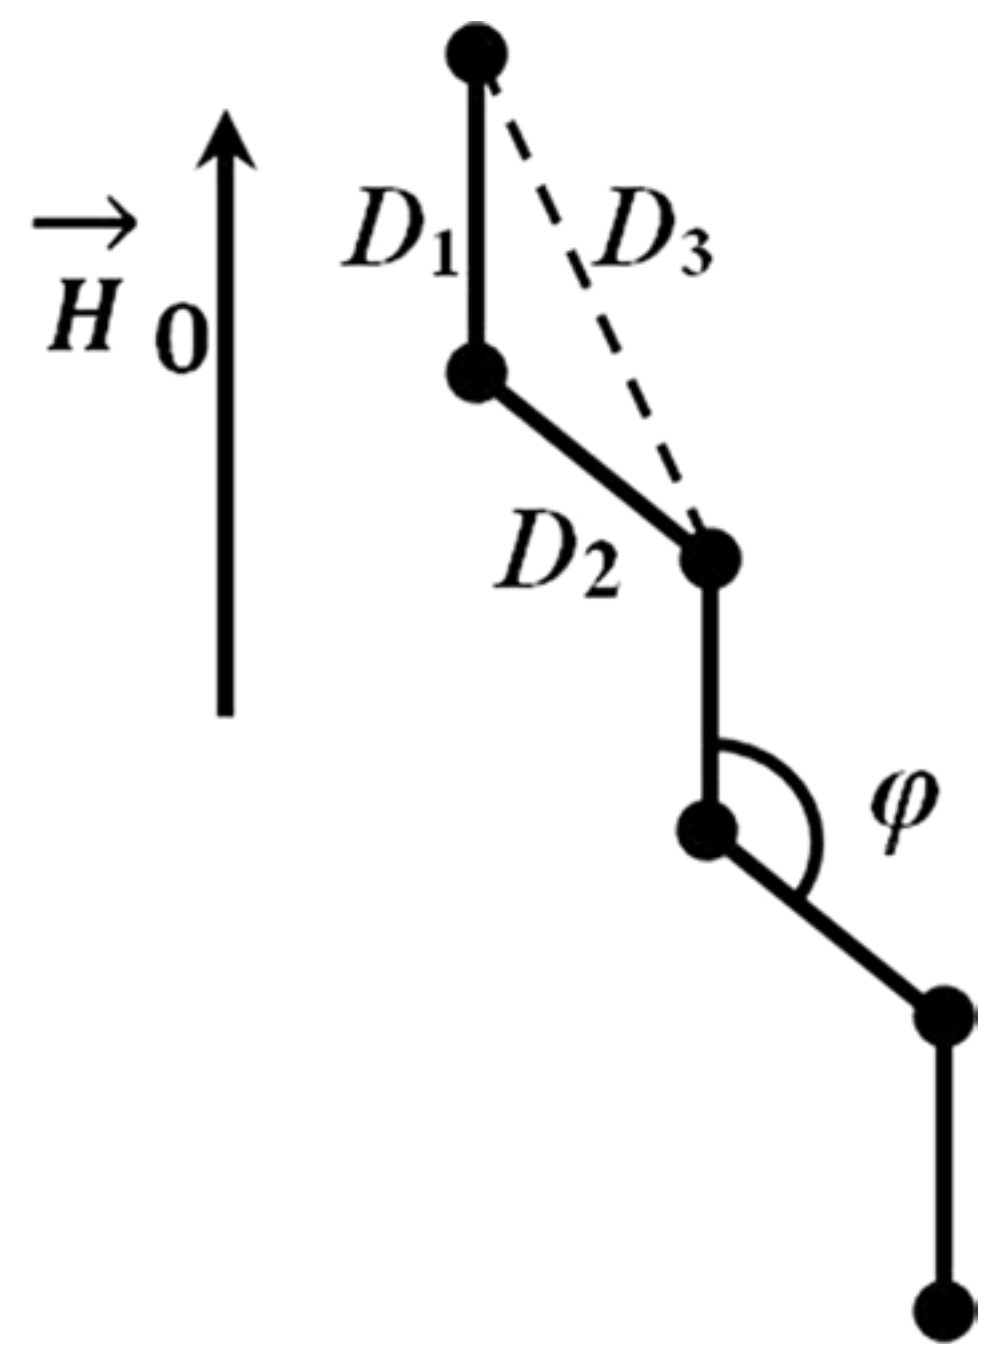
\includegraphics[width=0.5\textwidth]{model-zigzag-chain-schema.png}
%   \caption{Схема зигзагообзаной цепочки}
% \end{figure}
%
%     Константы взаимодействия
%         $$D_1=\dfrac{\gamma^2\hbar }{r^3}, $$
%         $$D_2 = D_1\dfrac{ 3\cos^2 \varphi -1 }{2} $$
%         $$D_3 = D_1 \dfrac{ 3\sin^2 \frac{\varphi}{2} -1}{16 \sin^3, \frac{\varphi}{2}}$$
%         где $\gamma$ - гиромагнитное отношение,
%         $\varphi$ - угол между соседними связями,
%         $r$ - расстояние между соседними спинами в цепочке.
%
%     Базовый случай это когда одна линия связи направлена вдоль поля. тогда констаты будет самой большой в доль поля.
%     Изменяя угол к полю мы можем получить как альтернированную цепочку так и однородную.
%     В приближении ближайших и следующих соседей, задача решается аналитически, но она
%     не дает полной картины. Поэтому мы решали данную систему численно.
%
%     \begin{figure}
%       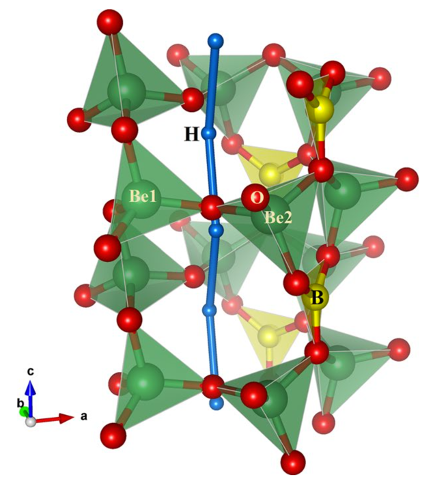
\includegraphics[width=0.85\textwidth]{model-zigzag-chain-hambergite-structure.png}
%       \caption{Hанопора со спин-несущих молекулами во внешнем сильном магнитном поле $\vec B$}
%     \end{figure}
%
%     Гамбергит $Be_2BO_3(OH)$
%         \begin{itemize}
%             \item Дипольное взаимодействия между ближайшими спинами протонов в цепи в 17 раз сильнее, чем со спинами окружающих цепей (в худшем случае).
%             \item Взаимодействия с остальными окружающими спинами по меньшей мере в 30 раз слабее.
%             \item Вклад дипольной связи между спинами в одной и той же цепи доминирует над остальными взаимодействиями.
%         \end{itemize}
%
%     В одномерных цепочках возникают когерентности только $\pm 2$ порядка
%     и следовательно дисперсия распределения будет небольшой
%     и мы не увидим запутанных кластеров.
%     Однако в альтернированная цепочке гамбергита возникают когерентности $\pm 4$ порядка
%     и следовательно можно использовать эту модель для исследования многочастичной запутанности.
%     The distance to these two protons is 4.49~\r{A}
%     The distance between a given chain and surrounding proton chains is at least 2.1 times larger than the distance between neighbors in the chain.
%

В предыдущей главе~\ref{chapter:manyparticle-entanglement-in-nanopore}
была подробно исследована многочастичная запутанность,
возникающая в МК эксперименте ЯМР в нанопоре.
Данная модель показала себя отличной площадкой
для исследования запутанности многих взаимодействующих частиц.
Тем не менее одномерные модели значительно лучше изучены как теоретически,
так и экспериментально~(см. раздел~\ref{sec:model-uniform-chain}).
В этой главе будет исследована многочастичная запутанность возникающая в таких системах.


\section{Однородная цепочка}
Однородная цепочка является наиболее простой разновидностью одномерной системы.
Создание запутанных кластеров в таких цепочках ограничено слабыми ДДВ удаленных спинов.
В МК эксперименте ЯМР в однородной цепочке возникают когерентности только нулевого и плюс/минус второго порядков.
Оценка снизу информации Фишера может быть получена с помощью Гауссова приближения для распределения интенсивностей МК когерентностей~\cite{Baum1985}.
В этом случае выражение для МК когерентностей имеет
%
\begin{equation}\label{eq:gaussaprox}
  J(\tau, T)=\dfrac{1}{\sqrt{\pi N_c(T)}} \exp\p{-\frac{n^2}{N_c(T)}},
\end{equation}
%
где $N_c(T)$ -- число коррелированных спинов,
ответственных за создание профиля МК когерентности.
Поскольку удвоенный второй момент интенсивностей МК когерентностей $2M_2(\tau, T)$ является нижней границей квантовой информации Фишера $F_Q$
(см.~раздел~\ref{sec:quantum-fisher-information-mesuarement-at-high-temperature}),
из уравнения~(\ref{eq:gaussaprox}) можно найти, что
%
\begin{equation}\label{eq:qfisheinf}
  F_Q \geq 2M_2(\tau, T) = N_c(T) \geq N,
\end{equation}
%
где $N$ --- число узлов в цепочке.
Для небольших значений $k$ верхнюю границу информации Фишера $k$-сепарабельного состояния
$F^k_Q = \sup{F_Q\p{\rho_{k-\mathrm{prod}}}}$~(см.~раздел.~\ref{sec:manyparticle-entanglement-criteria}) можно переписать в приближённой форме как
%
\begin{equation}\label{eq:inequalityforfq2}
  F^k_Q \leq k N.
\end{equation}
%
Неравенство~(\ref{eq:inequalityforfq2}) не нарушается ни для какого $k > 0$, когда $F_Q = N$,
а для случая $F_Q > N$ детектируется только парная запутанность.
Полученная оценка согласуется с представленными в литературе~\cite{Doronin2007, Feldman2012} результатами.

Из выражения~(\ref{eq:qfisheinf}) также следует,
что увеличение числа узлов цепочки не способствует детектированию запутанных кластеров большего размера, чем двухчастичный.
Тем не менее этого достаточно для передачи МК когерентностей вдоль цепочки~\cite{Bochkin2018qip} и создания запутанности между удаленными концами цепочки~\cite{Lazarev2019}.

% \subsection{Температурная зависимость запутанности удаленных узлов цепочки}
\subsection{Запутанность удаленных узлов цепочки}
\label{subsec:entanglement-of-remote-chain-nodes}
Однородная цепочка является удобной моделью линии связи для передачи квантовых состояний на короткие расстояния.
Типичная схема линии связи (см.~Рис.\ref{fig:model-uniform-chain-schema}) состоит из передатчика (sender $S$),
приемника (reciever $R$)
и линии передачи (transmition line $TL$).
Также ряд протоколов передачи задействуют расширенный приемник (extended reciever $ER$),
на котором применяется специально сконструированное универсальное унитарное преобразование для наилучшего восстановления передаваемой информации~\cite{Feldman2021}.

\begin{figure}[H]
  \centering
  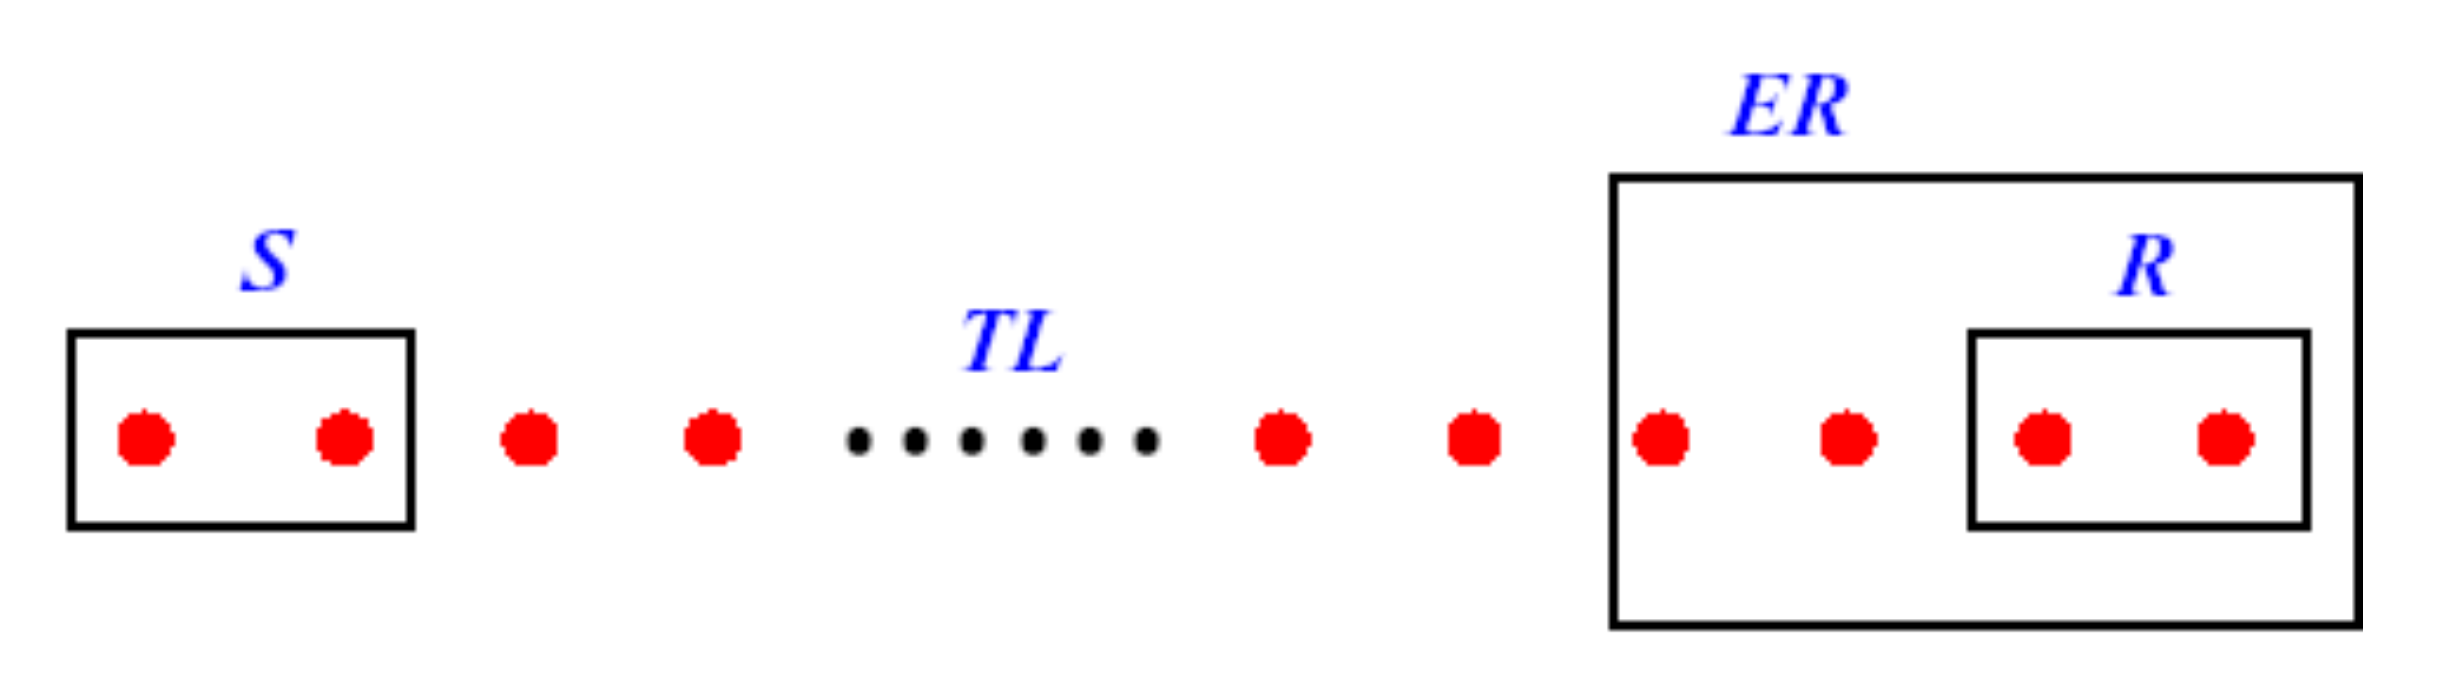
\includegraphics[width=0.9\textwidth]{model-uniform-chain-schema.png}
  \caption{
    Схематичное изображение линии передачи квантовых состояний.
    S --- передатчик,
    TL --- линия передачи,
    ER --- расширенный приемник,
    R --- приемник.
  }
  \label{fig:model-uniform-chain-schema}
\end{figure}

В оригинальной работе Бозе~\cite{Bose2003} был рассмотрен случай передачи однокубитного состояния под действием Гейзенберговского Гамильтониана.
В рамках МК спектроскопии ЯМР более естественно рассматривать передачу под действием $XX$-Гамильтониана,
который для однородной цепочки совпадает с МК Гамильтонианом $H_\mathrm{MQ}$~(\ref{eq:hmq}) с точностью до поворота~(см.~раздел~\ref{sec:model-uniform-chain}).
В приближении ближайших соседей во вращающейся системе координат с Ларморовской частотой $\omega_0$ выражение $XX$-Гамильтониана имеет вид:
%
\begin{equation}\label{eq:hxx}
  H_\mathrm{XX} = D\sum_{j=1}^{N-1}\p{I_{j,x}I_{j+1,x} + I_{j,y}I_{j+1,y}},
\end{equation}
где $D$ --- константна ДДВ между соседними узлами,
а N --- число узлов в цепочке.
В базисе бесспиновых фермионных операторов $\gamma_j$ and $\gamma_j ^+$
гамильтониан~(\ref{eq:hxx}) имеет диагональный вид
\begin{equation}\label{Diagonal_Hamiltonian}
  H_\mathrm{XX}=\sum\limits _{k}\varepsilon _{k}\gamma ^{+}_{k}\gamma _{k}.
\end{equation}
Переход к новому базису определяется преобразованием Йордана-Вигнера~\cite{Jordan1928, Feldman1998}:
\begin{equation}\label{eq:jw_operators}
  \gamma _{k}=\sum\limits ^{N}_{j=1}g_{kj} c_{j},
  \quad
  \gamma^+ _{k}=\sum\limits ^{N}_{j=1}g_{kj} c_{j}^+,
\end{equation}
где операторы рождения/уничтожения
\begin{equation}\label{eq:creation_annihilation_operators}
  c_{j}=(-2)^{j-1}I_{1,z}I_{2,z}I_{3,z}...I_{j-1,z}I^-_j,
  \quad
  c_{j}^+=(-2)^{j-1}I_{1,z}I_{2,z}I_{3,z}...I_{j-1,z}I^+_j,
\end{equation}
и
\begin{equation}\label{eq:gammakj}
  \varepsilon_{k} = D \cos(k),
  \quad
  g_{kj} =\sqrt {\frac {2}{N+1}}\sin \left( kj\right),
  \quad
  k=\frac {\pi n}{N+1}\quad n=1\ldots N .
\end{equation}

В общем случае в начальный момент времени однокубитный передатчик --- это произвольное чистое состояние
%
\begin{equation}\label{eq:random-pure-state}
  \ket{\psi_\mathrm{init}} = a\ket{0} + b\ket{1},
  \quad
  |a|^2 + |b|^2 = 1,
\end{equation}
%
а линия передачи и приемник находятся в термодинамическом равновесном состоянии
%
\begin{equation}
    \rho^\mathrm{TL, R}_\mathrm{init} = \otimes_{i=2}^N e^{\beta I_{i, z}}.
\end{equation}

Эволюционная матрица плотности может быть найдена из стационарного уравнения Лиювилля
\begin{equation}\label{eq:eval-rho-liuville}
  \rho(t) = e^{-iH_\mathrm{XX}t}
    \ket{\psi_\mathrm{init}} \bra{\psi_\mathrm{init}}
    \otimes
    \rho^\mathrm{TL, R}_\mathrm{init}
    e^{iH_\mathrm{XX}t}.
\end{equation}
После проведения редукции эволюционной матрицы плотности $\rho(t)$~(\ref{eq:eval-rho-liuville}),
матрица плотности передатчика и приемника определяется выражением
%
\small
\begin{equation}\label{eq:eval-rho-sr}
\rho^\mathrm{S,R}(t) =
\begin{pmatrix}
  \begin{array}{r}
    L(|f|^2+|g|^2) \\
    + \frac{e^{2\beta}}{(e^{\beta}+1)^2}
  \end{array}
  &
  \begin{array}{r}
    -\p{-\tanh\frac{\beta}{2}}^{N-2} \\
    \times \frac{ab^*f^* e^{\frac{\beta}{2}}}{2\cosh\frac{\beta}{2}}
  \end{array}
  &
  \frac{ab^* e^{\beta /2}}{2\cosh\frac{\beta}{2}}g^*
  &
  0\\
  &
  &
  &\\
  \begin{array}{r}
    -\p{-\tanh\frac{\beta}{2}}^{N-2} \\
    \times\frac{a^*bf e^{\frac{\beta}{2}}}{2\cosh\frac{\beta}{2}}
  \end{array}
  &
  \begin{array}{r}
    L(e^{-\beta}|g|^2-|f|^2) \\
    +\frac{1}{2\cosh{\beta}+2}
  \end{array}
  &
  \begin{array}{r}
    {2\p{-\tanh\frac{\beta}{2}}^{n-2}}\\
    \times Lfg^*\cosh\frac{\beta}{2}
  \end{array}
  &
  \frac{ab^* e^{-\beta/2}}{2\cosh\frac{\beta}{2}}g^* \\
  &
  &
  &\\
  \frac{a^*b e^{\beta /2}}{2\cosh\frac{\beta}{2}}g
  &
  \begin{array}{r}
   2\p{-\tanh\frac{\beta}{2}}^{n-2}\\ \times{Lf^*g\cosh\frac{\beta}{2}}
  \end{array}
  &
  \begin{array}{r}
    L(e^{-\beta}|f|^2 -|g|^2) \\
    +\frac{1}{2\cosh{\beta}+2}
  \end{array}
  &
  \begin{array}{r}
    \p{-\tanh\frac{\beta}{2}}^{N-2} \\
    \times \frac{ab^*f^* e^{-\frac{\beta}{2}}}{2\cosh\frac{\beta}{2}}
  \end{array}
  &
  &
  &\\
  0
  &
  \frac{a^*b e^{-\beta /2}}{2\cosh\frac{\beta}{2}}g
  &
  \begin{array}{r}
    \p{-\tanh\frac{\beta}{2}} ^{N-2} \\
    \times \frac{a^*bf e^{-\frac{\beta}{2}}}{2\cosh\frac{\beta}{2}}
  \end{array}
  &
  \begin{array}{r}
    -L e^{-\beta}(|f|^2 +|g|^2)\\
    + \frac{1}{(e^{\beta}+1)^2}
  \end{array}
\end{pmatrix},
\end{equation}
\normalsize
где $f={f_N(t, N)}$, $g={f_N(t, 1)}$, $L=\frac{1-2|b|^2 e^{\frac{\beta}{2}}\cosh\frac{\beta}{2}}{\cosh\frac{\beta}{2}}$
и
%
\begin{equation}
  f_N(t, j) = \frac{2}{N+1}\sum_k e^{i\epsilon_k t}\sin k \sin jk.
\end{equation}

\begin{figure}[H]
  \begin{subfigure}{0.45\textwidth}
    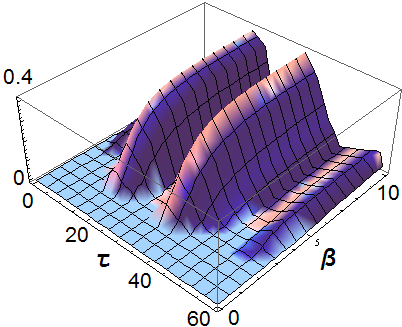
\includegraphics[width=\textwidth]{concurence-temp-uniform-chain-N4.png}
    \caption{
      $\ket{\psi} = \dfrac{\ket{0} + \ket{1}}{\sqrt{2}}$
    }
    \label{fig:concurence-temp-uniform-chain-N4}
  \end{subfigure}
  \hfill
  \begin{subfigure}{0.45\textwidth}
    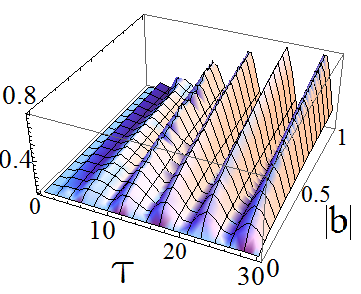
\includegraphics[width=\textwidth]{concurence-polarization-uniform-chain-N4.png}
    \caption{
      $\beta = 5$
    }
    \label{fig:concurence-polarization-uniform-chain-N4}
  \end{subfigure}
  \caption{
    Зависимость согласованности $C$ от безразмерного времени $\tau = Dt$,
    обратной температуры $\beta$
    (cм. Рис.~\ref{fig:concurence-temp-uniform-chain-N4})
    и величины поляризации $|b|$
    (cм. Рис.~\ref{fig:concurence-polarization-uniform-chain-N4})
    при передаче квантового состояния по цепочке из $N=4$ спинов.
  }
  \label{fig:councurence-uniform-chain-N4}
\end{figure}

В качестве критерия запутанности для двухкубитного смешанного состояния удобнее всего использовать критерий Вуттерса~(см. раздел. ~\ref{sec:entanglement-criteria}) на основе согласованности $C$.
Температурная зависимость согласованности $C$ при передаче чистого состояния $\ket{\psi} = \frac{\ket{0} + \ket{1}}{\sqrt{2}}$ ($a=b=\frac{1}{\sqrt{2}}$) представлена на Рис.~\ref{fig:concurence-temp-uniform-chain-N4}.
При обратной температуре $\beta > 1$ приемник и передатчик запутываются.
На Рис.~\ref{fig:concurence-polarization-uniform-chain-N4} представлена зависимость согласованности $C$ от различных значений начальной поляризации передатчика при температуре $\beta = 5$.
Приемник и передатчик запутываются при любой начальной поляризации.

\begin{figure}[H]
    \centering
    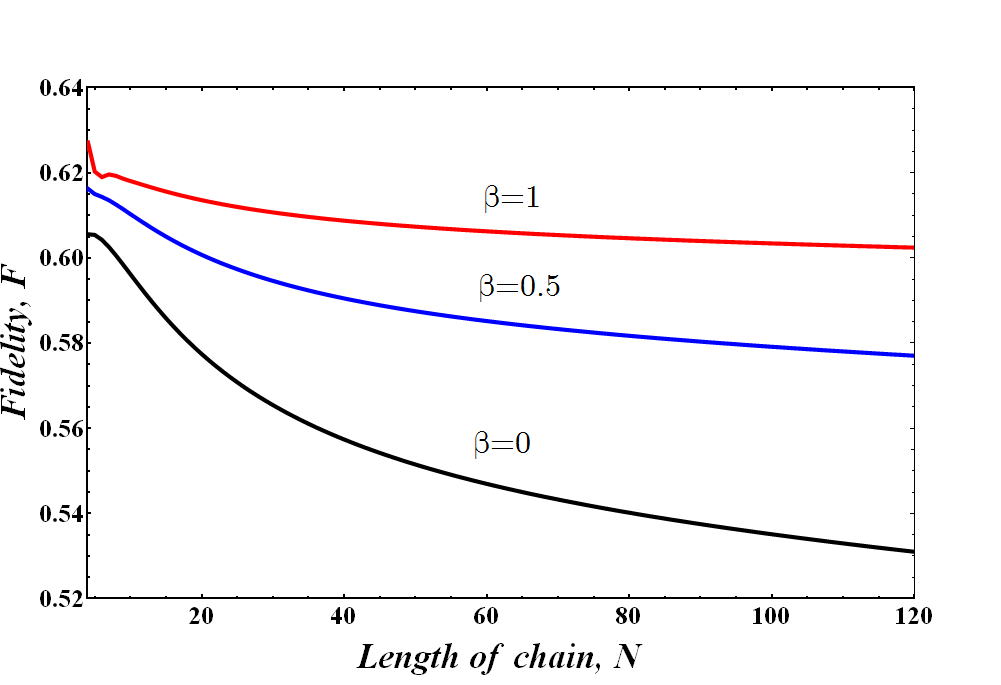
\includegraphics[width=0.8\textwidth]{fidelity-n-beta.png}
    \caption{
      Зависимость фиделити переданного состояния
      $\rho^\mathrm{S}_\mathrm{init}$
      и полученного
      $\rho^\mathrm{R}\p{\bar\tau_N}$
      от количества узлов в цепи.
      Разные линии соответствуют разным значениям обратной температуры $\beta$.
     }
    \label{fig:fidelity-n-beta}
\end{figure}

Идеальная передача произвольного квантового состояния в спиновых цепочках достижима только в очень специфических случаях~\cite{Christandl2004, Karbach2005} и может быть легко разрушена небольшими возмущениями гамильтониана взаимодействия.
В общем случае передача осуществляться не идеально,
но с высокой вероятностью.
Качество передачи можно оценить с помощью фиделити~\cite{Jozsa1994}
%
\begin{equation}\label{generalFidelity}
  F\p{\rho^\mathrm{S}_\mathrm{init}, \rho^\mathrm{R}\p{t}}
  = \tr{\rho^\mathrm{S}_\mathrm{init}, \rho^\mathrm{R}(t)}.
\end{equation}
%
С учетом $\rho^\mathrm{R}\p{t} = \tr{\rho^\mathrm{S,R}(t)}_\mathrm{S}$,
аналитическое выражение для фиделити имеет вид
%
\begin{multline}\label{exactfidelity}
  F\p{\rho^\mathrm{S}_\mathrm{init}, \rho^\mathrm{R}\p{t}}
  = (1-2|b|^2)\p{
    \frac{e^{\beta/2}}{\cosh \beta/2}
    + \p{\frac{e^{-\beta/2}}{\cosh \beta/2} -|b|^2 }
      \left|f_N(t, N)\right|^2
  } \\
  + |b|^2
  + 2 |b|^2 \p{1-|b|^2} \Re\left\{f_N(t, N)\right\}
  \p{-\tanh \p{\frac{\beta}{2}}}^{N-1}.
\end{multline}
%
Время $\bar\tau_{N}$, при котором фиделити достигает первого пика, называется временем передачи~\cite{Feldman2016}.
Оно совпадает с временем первого пика функции $\left|f_N(t, N)\right|^2$.
Фиделити~\cite{Jozsa1994} переданного и полученного квантового состояния в момент времени $\bar\tau_{N}$ уменьшается с увеличением длинны цепочки (см. Рис.\ref{fig:fidelity-n-beta}).


\subsection{Идеальная передача запутанных состояний}
% \subsection{Идеальная передача МК когерентности нулевого порядка}

Гамильтониан $H_\mathrm{XX}$ коммутирует с $z$-проекцией $I_z$ полного спинового момента
и сохраняет число возбуждений в процессе эволюции.
В этом случае когерентности разных порядков не перемешиваются~\cite{Feldman2017} и могут быть рассмотрены отдельно~\cite{Bochkin2018qip}.
В частности, было показано~\cite{Feldman2021},
что специальная форма когерентности нулевого порядка может передаваться без потерь
по цепочке из $N$ узлов, находящейся в основном состоянии:
%
\begin{equation}
  \rho^\mathrm{TL}_\mathrm{init} = \otimes^{N_\mathrm{TL}}_{i=1}\ket{0},
  \quad
  \rho^\mathrm{R}_\mathrm{init} = \otimes^{N_\mathrm{R}}_{i=1}\ket{0},
\end{equation}
%
где $N_\mathrm{R}$ --- количество кубитов в приёмнике,
а $N_\mathrm{TL}  = N - 2 N_\mathrm{R}$.
В случае, когда количество кубитов в передатчике $N_\mathrm{S} = N_\mathrm{R} = 3$,
специальная матрица плотности передатчика,
которая может быть передана без потерь,
в базисе с одним возбуждением
$\left \{\ket{000}, \ket{001}, \ket{010}, \ket{100} \right\}$
может быть записана в виде
%
\begin{equation}
  \rho^\mathrm{S}_\mathrm{init} =
  \begin{pmatrix}
    u &    0     &    0    & 0 \\
    0 &   x_1    & \omega  & 0 \\
    0 & \omega^* &   x_2   & 0 \\
    0 &    0     &    0    & v
  \end{pmatrix}.
\end{equation}
%
После редукции $\rho^\mathrm{S}_\mathrm{init}$ по первому спину
матрица плотности оставшихся двух в полном базисе имеет вид
\begin{equation}\label{eq:rho-s-reduced}
  \tr{\rho^\mathrm{S}_\mathrm{init}}_{1} =
  \begin{pmatrix}
    u + v &    0     &    0    & 0 \\
    0     &   x_1    & \omega  & 0 \\
    0     & \omega^* &   x_2   & 0 \\
    0     &    0     &    0    & 0
  \end{pmatrix}.
\end{equation}
Для матрицы вида~(\ref{eq:rho-s-reduced}) согласованность $C$
определяется~(cм.~раздел~\ref{sec:entanglement-criteria}) только величиной недиагональных элементов:
%
\begin{equation}
  C = 2 |w|.
\end{equation}


\begin{figure}[H]
    \centering
    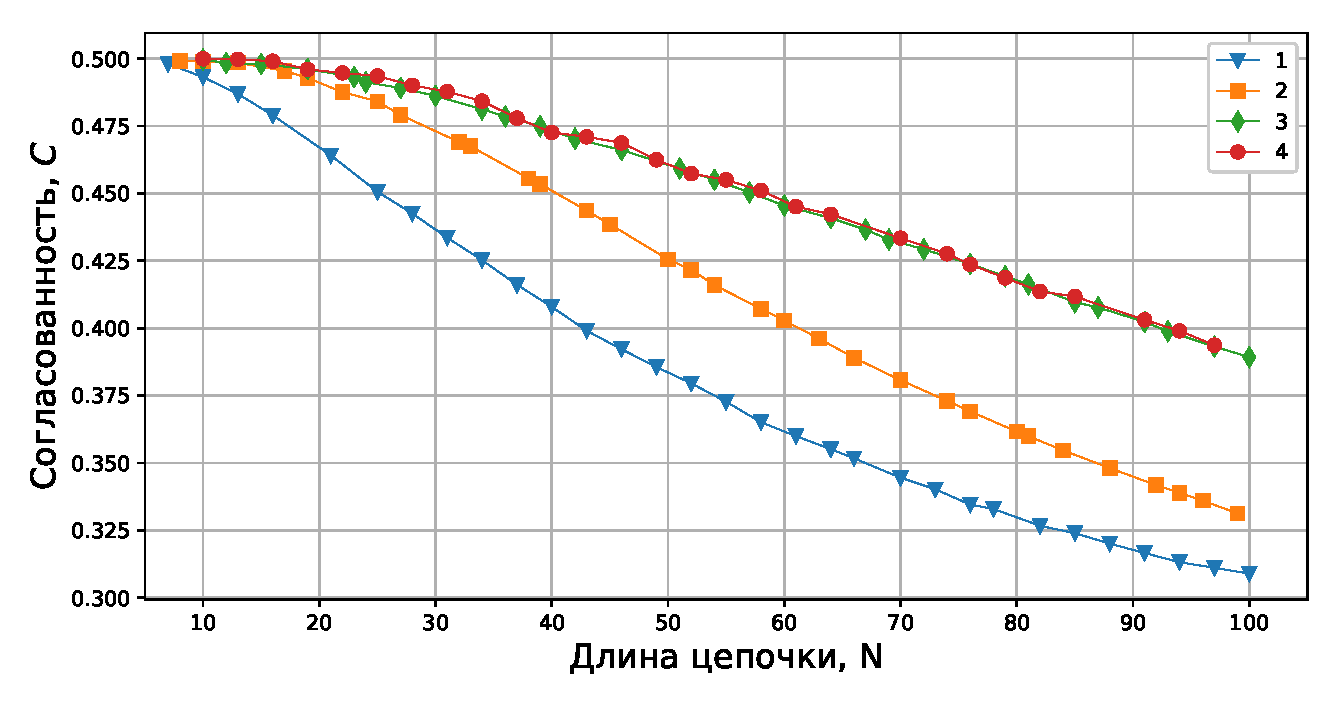
\includegraphics[width=0.9\textwidth]{concurence-n-s3.eps}
    \caption{
      Максимальное значение согласованности второго и третьего спинов передатчика, состояние которого может быть передано без потерь,
      от количества узлов в цепи.
      Разные линии отвечают разным размерам расширенного приемника.
    }
    \label{fig:concurence-n-s3}
\end{figure}


Так как элементы матрицы плотности, вносящие вклад в каждую когерентность, перемешиваются в процессе эволюции,
на расширенном приемнике ER применятся специальное унитарное преобразование $U^\mathrm{ER}(\phi)$ для их распутывания~\cite{Feldman2017}.
По аналогии с работой~\cite{Bochkin2022} можно подобрать такое унитарное преобразование на расширенном приемнике,
которое позволяет передавать состояния с максимальным значением согласованности второго и третьего спинов передатчика.
На Рис.~\ref{fig:concurence-n-s3} приведены максимально возможные значения согласованности от длины цепочки,
полученные путем максимизации модуля недиагонального элемента $\omega$ матрицы плотности $\rho^\mathrm{S}_\mathrm{init}$ по параметрам унитарного преобразования $U^\mathrm{ER}(\phi)$.
Вычисления выполнены с помощью метода дифференциальной эволюции~\cite{Storn1997,Wormington1999,Lampinen2002} из библиотеки SciPy~\cite{SciPy} версии 1.4.1.


\section{Зигзагообразная цепочка}
В зигзагообразных цепочках в кристалле гамбергита в МК эксперименте ЯМР,
в отличие от однородных цепочек,
возникают когерентности плюс/минус четвертого порядка (см. раздел~\ref{sec:model-zigzag-chain}).
Данное обстоятельство является важным для исследования многоспиновой запутанности,
поскольку при этом используется второй момент распределения МК когерентностей ЯМР.

\begin{figure}[H]
    \centering
    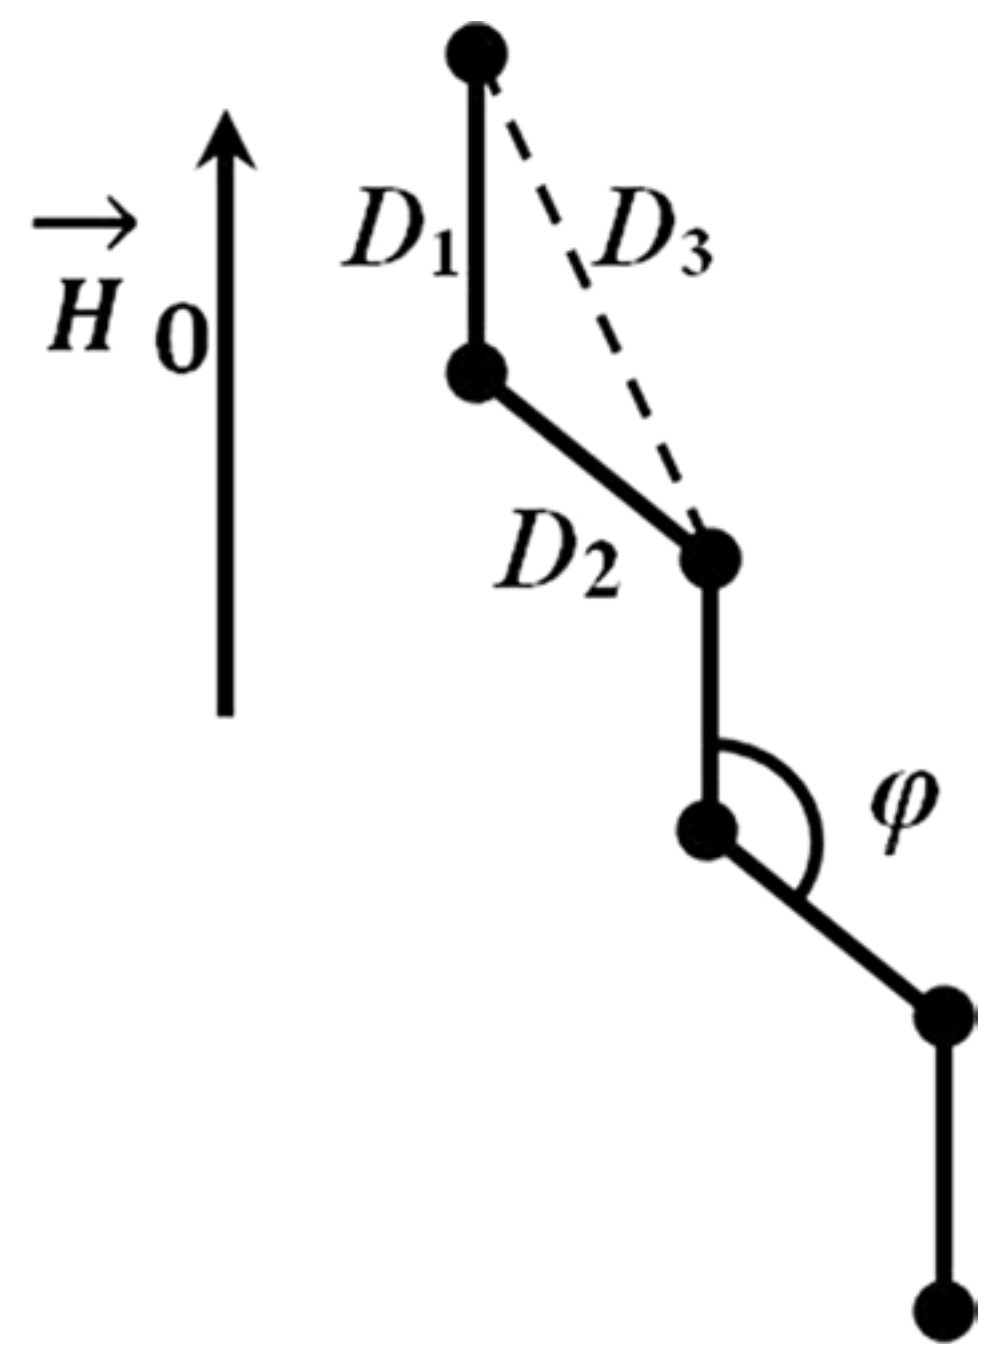
\includegraphics[width=0.3\textwidth]{model-zigzag-chain-schema}
    \caption{
      Зигзагообразная цепочка ядерных спинов.
      Нечетные звенья параллельны внешнему магнитному полю $\vec{\mathcal H}_0$,
      а $\varphi$ - угол между соседними звеньями.
      Константы связи $D_1$ и $D_2$ определяются уравнением~(\ref{eq:dipolaconstantsnearest}), а $D_3=D_{n, n+2},\, (n=1,2,...)$
      уравнением~(\ref{eq:dipolaconstantsnextnearest}).
    }
    \label{fig:model-zigzag-chain-schema}
\end{figure}

На Рис.~\ref{fig:model-zigzag-chain-schema} схематично представлена
зигзагообразная цепочка ядерных спинов в сильном внешнем магнитным полем $\vec{\mathcal H}_0$.
Нечетные звенья цепочки параллельны внешнему магнитному полю $\vec{\mathcal H}_0$,
а $\varphi$ - угол между соседними звеньями.
Гамильтониан $H_\mathrm{MQ}$,
описывающий МК динамику ЯМР~(см. раздел~\ref{sec:mq-nrm-experiment}),
задается выражением~\cite{Doronin2000}
%
\begin{equation}\label{hmqnextnearest}
 H_\mathrm{MQ} = \sum_{i=1}^{N-1} D_{i, i+1}(I_i^{+}I_{i+1}^{+}+ I_i^{-}I_{i+1}^{-} )
   + \sum_{i=1}^{N-2} D_{i, i+2}(I_i^{+}I_{i+2}^{+}+ I_i^{-}I_{i+2}^{-} ) ,
\end{equation}
%
где $I_i^+$, $I_i^-$ --- это повышающей и понижающий операторы спинового углового момента спина с номером $i$,
и $N$ --- это количество ядерных спинов в цепочке.

Константы диполь-дипольного взаимодействия (ДДВ)
в зигзагообразной цепочке определяются выражениями~\cite{Abragam1982}
%
\begin{equation}\label{eq:dipolaconstantsnearest}
  D_{2n-1, 2n} = D_1 =\dfrac{\gamma^2\hbar }{r^3},
  \quad
  D_{2n, 2n+1} = D_2=\dfrac{\gamma^2\hbar }{2r^3}\p{3\cos^2 \varphi -1},
  \quad
  n=1,2\dots,
\end{equation}
где $\gamma$ -- гиромагнитное отношение,
и $r$ -- расстояние между ближайшими спинами в цепочке.
Также в гамильтониане учитываются взаимодействия со следующими соседями,
константа диполь-дипольного взаимодействия которых определяется как~\cite{Abragam1982}
%
\begin{equation}\label{eq:dipolaconstantsnextnearest}
  D_{n, n+2}=\dfrac{\gamma^2\hbar }{16r^3 \sin^3 \frac{\varphi}{2}}\p{3\sin^2 \frac{\varphi}{2} -1}.
\end{equation}
%
В частности, уравнения~(\ref{eq:dipolaconstantsnearest}),~(\ref{eq:dipolaconstantsnextnearest}) означают,
что для прямой спиновой цепочки, когда  $(\varphi=\pi)$,
константа дипольной связи для ближайших соседей в восемь раз больше,
чем константа дипольной связи между следующими ближайшими соседями.
Тем не менее при $\varphi=\frac{2\pi}{3}$ отношение констант связи
\begin{equation}
  \left|\dfrac{D_{2n, 2n+1}}{D_{2n-1, 2n+1}}\right| = \dfrac{3\sqrt{3}}{5},
\end{equation}
и, следовательно,
диполь-дипольные взаимодействия следующих ближайших соседей
существенны для МК динамики ЯМР при определённых ориентациях зигзагообразной спиновой цепочки
по отношению к направлению внешнего сильного магнитного поля.


\subsection{Температурная зависимость многочастичной запутанности}
Для исследования температурной зависимости многочастичной запутанности
в зигзагообразных цепочках
в этом разделе будет рассмотрена МК динамика ЯМР
на подготовительном периоде МК эксперимента ЯМР~(см. раздел~\ref{sec:mq-nrm-experiment})
с начальным термодинамически равновесным состоянием $\rho_\mathrm{eq}$.
Матрица плотности системы в начальный момент времени имеет вид:
\begin{equation}
  \rho(0, \beta)
  = \rho_\mathrm{eq}
  = \dfrac{e^{\frac{\hbar\omega_{0}}{kT} I_z}}{Z},
  = \dfrac{e^{\beta I_z}}{Z},
\end{equation}
где $Z = \tr{e^{\beta I_z}}$ --- статистическая сумма,
$\hslash$ и $k$ --- константы Планка и Больцмана,
$\omega_{0}$ --- частота Лармора,
$I_\mathrm{z}$ ---  оператор проекции полного углового спинового момента  на ось~$z$,
который направлен вдоль сильного внешнего магнитного поля.

Интенсивности приведенных МК когерентностей ЯМР определяются уравнением~\ref{eq:reduced-mq-coherences}~(см. раздел~\ref{sec:reduced-mq-coherences}).
Для $b=0.5$,
что соответствует температуре $T=4.8 \times 10^{-2}\,\mbox{K}$
при Ларморовской частоте $\omega_0=2\pi\times 500\times 10^6 \,\mbox{s}^{-1}$,
было обнаружено,
что неравенство~(\ref{eq:entanglement-criteria}) может быть выполнено только при $k=1$ для спиновых цепочек с $N=6$ и $N=8$.
Это означает, что в высокотемпературном случае~\cite{Doronin2019}
детектируется парная запутанность,
что согласуется с работой~\cite{Feldman2012}.

\begin{figure}[H]
  \begin{subfigure}[t]{0.49\textwidth}
    
\includegraphics[width=\textwidth]{m2-by-time-in-zigzag-chain-with-n6-beta10}
    \caption{
      Зависимость нижней границы квантовой информации
      Фишера~$F_Q=2M_2(\tau, T)$
      от безразмерного времени~$D_1\tau$
      для зигзагообразной цепочки из 6 спинов
      при температуре $2.4\times 10^{-3}\,\mbox{K}$ $(b=10)$.
      В области выше горизонтальной линии $k=1$
      гарантировано существует как минимум парная запутанность.
      В области выше горизонтальной линии $k=5$
      гарантировано существует шестиспиновая запутанность.
    }
    \label{fig:fig3}
  \end{subfigure}
  \hfill
  \begin{subfigure}[t]{0.49\textwidth}
    
\includegraphics[width=\textwidth]{nent-by-n-b10}
    \caption{
      Зависимость оценки максимального количества запутанных спинов $N_{ent}$ от длины цепочки при температуре $2.4\times 10^{-3}\,\mbox{K}$.
    }
    \label{fig:fig4}
  \end{subfigure}
  \caption{}
\end{figure}

Зависимости многоспиновой запутанности от длины цепочки $N$ и температуры исследованы для спиновых цепочек с $4\leqslant N \leqslant 12$.
Временная эволюция нижней границы квантовой информации Фишера,
соответствующая  удвоенному второму моменту распределения интенсивностей МК когерентностей для шестиспиновой цепочки представлена на Рис.~\ref{fig:fig3} при температуре $2.4\times 10^{-3}\,\mbox{K}$ $(b=10)$.
На Рис.~\ref{fig:fig3} видна полоса,
в которой неравенство~(\ref{eq:entanglement-criteria}) может быть удовлетворено при $1\leqslant k \leqslant 5$.
Таким образом, существует многоспиновая запутанность в спиновых кластерах, состоящих из 2-6 спинов при температуре $2.4\times 10^{-3}\,\mbox{K}$.
Зависимость оценки максимального количества запутанных спинов от длины цепи приведена на Рис.~\ref{fig:fig4} при температуре $2.4\times 10^{-3}\,\mbox{K}$.

\begin{figure}[H]
  \begin{subfigure}[t]{0.49\textwidth}
    
\includegraphics[width=\textwidth]{m2-by-time-in-zigzag-chain-with-n8-beta1}
    \caption{
      При температуре $2.4\times 10^{-2}\,\mbox{K}$
      в области ограниченной горизонтальными линиями $k=1$ и $k=2$
      присутствует как минимум парная запутанность.
    }
    \label{fig:fig5}
  \end{subfigure}
  \hfill
  \begin{subfigure}[t]{0.49\textwidth}
    
\includegraphics[width=\textwidth]{m2-by-time-in-zigzag-chain-with-n8-beta10}
    \caption{
       При температуре $1.2\times 10^{-3}\,\mbox{K}$
       в области ограниченной горизонтальными линиями $k=2$ и $k=4$
       наблюдается как минимум трехчастичная запутанность.
    }
    \label{fig:fig6}
  \end{subfigure}
  \caption{
    Временная эволюция нижней границы информации Фишера~$F_Q=2M_2(\tau, T)$
    от безразмерного времени~$D_1\tau$
    в восьмиспиновой зигзагообразной цепочке.
  }
\end{figure}

Временная эволюция восьмиспиновой зигзагообразной цепочки представлена при $T=2.4\times 10^{-2}\,\mbox{K}$ (Рис.~\ref{fig:fig5}) и $T=1.2\times 10^{-2}\,\mbox{K}$ (Рис.~\ref{fig:fig6}).  Видно, что при температуре $T=2.4\times 10^{-2}\,\mbox{K}$ возникают многоспиновые запутанные кластеры, состоящие из двух или трех спинов, а при температуре $T=1.2\times 10^{-2}\,\mbox{K}$ возникают кластеры с $2\leqslant k \leqslant 5$.
Число запутанных спинов увеличивается с понижением температуры.

\begin{figure}[H]
  \centering
  
\includegraphics[width=0.6\textwidth]{nent-by-beta-n8-n6}
  \caption{
    Зависимость оценки максимального числа запутанных спинов от обратной температуры $b$
    для зигзагообразной цепочки,
    состоящей из шести и восьми спинов.
    }
    \label{fig:fig7}
\end{figure}

Зависимость числа запутанных спинов от температуры для зигзагообразных цепочек,
состоящих из шести или восьми спинов, приведена на Рис.~\ref{fig:fig7}.
% В этих цепочках почти все спины запутаны при низких температурах.
Так же как и в случае системы эквивалентных спинов,
при низких температурах почти все спины в цепочке запутанны.
% Результаты получены на небольшом интервале времени,
% поэтому эффектами декогеренции можно пренебречь.


% The creation of entangled clusters in the considered zigzag chains is limited by weak DDIs of remote spins.  Accordingly, that process requires a large time interval. Practically, the role of decoherence gets very important in that case.  We note also that the analysis of the inequality \eqref{inequalityforfq} shows that an increase in chain length does not result in an increase of the number of the entangled spins even at long times. Indeed, we can rewrite \eqref{inequalityforfq} in the approximate simple form
% \begin{equation}\label{inequalityforfq2}
% F_Q>k N.
% \end{equation}
% In order to estimate the Fisher information we use the Gaussian approximation for the distribution of the intensities of MQ coherences \cite{baum}
% \begin{equation}\label{gaussaprox}
% J(\tau, T)=\dsfrac{1}{\sqrt{\pi N_c(T)}} \exp\p{{-\frac{n^2}{N_c(T)}}},
% \end{equation}
% where $N_c(T)$ is the number of the correlated spins which are responsible for the creation of the MQ coherence profile. Since twice the second moment $2M_2(\tau, T)$ is a lower bound on the quantum Fisher information $F_Q$ \cite{toth, pezze} one can find from Eq. \eqref{gaussaprox} that
% \begin{equation}\label{qfisheinf}
% F_Q=N_c(T).
% \end{equation}
% Since $N\geqslant N_c(T)$, one can conclude that in the Gaussian model \cite{baum} only two-spin entanglement is possible.
%
% Numerical calculations for the zigzag spin chain yield similar results. We find that the Fisher information depends only weakly on the number of spins. It means (see Eq. \eqref{inequalityforfq2}) that the number of the entangled spins decreases when $N$ increases. We have found that in the zigzag six-spin system all six spins can be entangled. On the contrary, only three spins are entangled in the zigzag ten-spin system.
%
% Finally, the number of the entangled spins for the zigzag chain with $4\leqslant N\leqslant 12$ increases with decreasing temperature.


\section{Выводы}
В этом разделе была исследована многочастичная запутанность
возникающая на подготовительном периоде МК эксперимента ЯМР
в зигзагообразной цепочке ядерных спинов.
Несмотря на то, что в одномерных системах
создание запутанных кластеров ограничено слабыми ДДВ удаленных спинов,
удалось показать что качественное поведение температурной зависимости многочастичной запутанности
в зигзагообразной цепочке совпадает с поведением в системе эквивалентных спинов.
%Несмотря на то, что одномерные системы демонстрируют
%более скромные оценки количества запутанных частиц
%из-за отсутствия сильных дальнодействующих связей,
%можно заключить,
%что качественное поведение температурной зависимости многочастичной запутанности
%совпадает с поведением в системе эквивалентных спинов.
Более того, полученные результаты исследования запутанности
соответствуют результатам, представленным в литературе.
Таким образом, можно заключить,
что разработанный в данной диссертации метод
является мощным инструментом для исследования многочастичной запутанности в любой системе.